%Packages and stuff

\documentclass[final,dvipsnames]{beamer}
%% Possible paper sizes: a0, a0b, a1, a2, a3, a4.
%% Possible orientations: portrait, landscape
%% Font sizes can be changed using the scale option.
\usepackage[size=a0,orientation=portrait,scale=1.4,debug]{beamerposter}
%\mode<presentation>{\usetheme{inriaposter}}
\usetheme{LLT-poster}
\usecolortheme{ComingClean}
%\usecolortheme{Entrepreneur}
%\usecolortheme{ConspiciousCreep}
\usepackage[utf8]{inputenc}
\usepackage[T1]{fontenc}
\usepackage{libertine}
\usepackage[scaled=1]{inconsolata}
%\usepackage[libertine]{newtxmath}
\usepackage{amsmath,amsfonts,amssymb,pxfonts,eulervm,xspace}
\usepackage{graphicx,subfigure,comment,tikz}
\usepackage{array}
\usepackage{adjustbox}
\usepackage{framed}
\usepackage{mdframed}
\usepackage{multirow}
\usepackage{xcolor}


%---------------------------------------

\addtobeamertemplate{block end}{}{\vspace*{2pt}}


%---------------------------------------------------------------------------------------%

%CUSTOM COMMANDS
\newcommand{\myemph}[1]{\textcolor{blue}{#1}}
\newcommand{\myemphh}[1]{\textbf{\textcolor{blue}{#1}}}
\newcommand{\myemphr}[1]{\textbf{\textcolor{red}{#1}}}
\newcommand{\myemphBLACK}[1]{\textcolor{black}{#1}}

\newcommand{\mycolbackwhite}[1]{
\hspace*{.01\linewidth}\begin{minipage}{.96\linewidth}
\begin{mdframed}[backgroundcolor=white!10,linewidth=3pt]
\vspace{10pt}
#1
\vspace{10pt}
\end{mdframed}
\end{minipage}
}

\newcommand{\mycolbackblue}[1]{
\hspace*{.01\linewidth}\begin{minipage}{.96\linewidth}
\begin{mdframed}[backgroundcolor=blue!10,linewidth=3pt]
\vspace{10pt}
#1
\vspace{10pt}
\end{mdframed}
\end{minipage}
}

\newcommand{\mycolbackred}[1]{
\hspace*{.01\linewidth}\begin{minipage}{.40\linewidth}
\begin{mdframed}[backgroundcolor=red!10,linewidth=3pt]
\vspace{10pt}
#1
\vspace{10pt}
\end{mdframed}
\end{minipage}
}

\newcommand{\mycolbackgreen}[1]{
\hspace*{.01\linewidth}\begin{minipage}{.35\linewidth}
\begin{mdframed}[backgroundcolor=green!10,linewidth=1pt]
\vspace{10pt}
#1
\vspace{10pt}
\end{mdframed}
\end{minipage}
}

\newcommand{\mycolbackgreenw}[1]{
\hspace*{.01\linewidth}\begin{minipage}{.96\linewidth}
\begin{mdframed}[backgroundcolor=blue!10,linewidth=1pt]
\vspace{10pt}
#1
\vspace{10pt}
\end{mdframed}
\end{minipage}
}



\DeclareMathOperator\supp{supp}
\DeclareMathOperator\argmin{argmin}
\DeclareMathOperator\Bern{Bern}


%---------------------------------------------------------------------------------------%
%Title, author, etc


\newcommand{\footleft}{martin.gjorgjevski@gipsa-lab.grenoble-inp.fr}
\newcommand{\footright}{\footnotesize This work was supported in part by blah blah}


\title{Graphical Nadaraya-Watson Estimator on Latent Position Models}
\author{Martin Gjorgjevski$^1$, Nicolas Keriven$^1$, Simon Barthelme$^1$, Yohann De Castro$^2$}
\institute{$^1$CNRS Gipsa-Lab, Grenoble, $^2$CNRS Ecole Centrale Lyon, Lyon}




%--------------------------------------------------------------------------------------%
%biblio
%\usepackage{natbib}
\bibliographystyle{IEEEbib}
% make bibliography entries smaller
%\renewcommand\bibfont{\scriptsize}
% Now get rid of all the colours
\setbeamercolor*{bibliography entry title}{fg=black}
\setbeamercolor*{bibliography entry author}{fg=black}
\setbeamercolor*{bibliography entry location}{fg=black}
\setbeamercolor*{bibliography entry note}{fg=black}

\setbeamertemplate{bibliography entry title}{}
\setbeamertemplate{bibliography entry location}{}
\setbeamertemplate{bibliography entry note}{}
\setbeamertemplate{bibliography item}{\insertbiblabel}





\usetikzlibrary{decorations.pathreplacing}





%------------------------------------------------------------------------
\begin{document}
\begin{frame}

\begin{block}{Summary}
    The \textit{\myemphh{Graphical Nadaraya Watson}} Estimator $\hat{f}_{GNW}$ is a signal averaging estimator on graphs, inspired by the \textit{\myemphr{Nadaraya-Watson Estimator}} $\hat{f}_{NW}$ in nonparametric estimation. 
    We study concentration properties and risk decay rates of $\hat{f}_{GNW}$ in terms of the growth of the degree of the node. Under mild assumptions on the signal, the estimator concentrates with a rate inversly proportional to the node degree, For smooth signals $\hat{f}_{GNW}$ and $\hat{f}_{NW}$ achieve similar risk rates.    
\end{block}    

\begin{columns}[T]

    

%%%% First Column
\begin{column}{0.49\textwidth}
\begin{block}{Framework: \textit{Latent Position Models}}
\begin{itemize}
\item $X_1,...X_n,X$ i.i.d. $\sim p$, $p$ a density on $\mathbb{R}^d$
\textit{not observed}
\vspace{10pt}
\item $k_n:\mathbb{R}^d\to [0,1]$ \textit{probability kernel} 
\vspace{10pt}
\item $a(X_i,X_j)=bern(k_n(X_i,X_j))$ \textit{edge between nodes $i$ and $j$}
\vspace{10pt}
\item $Y_i-f(X_i)+\epsilon_i$, $\epsilon=(\epsilon_i)_{i=1}^n$ \textit{noise independent from} $(X_i)_{i=1}^n$, with $\mathbb{E}\epsilon_i=0$, $\mathbb{E}\epsilon_i^2
=\sigma^2<\infty$ 
\vspace{10pt}
\item $d_n(x)=\mathbb{E}(\sum_{i=1}^n a(X,X_i)|X=x)$ \textit{local expected degree at $x$}
\end{itemize}
\vspace{20pt}
\mycolbackgreen{
    \textit{Goal: \textbf{Estimate} $f(X)$}
}
\begin{figure}
    \centering
    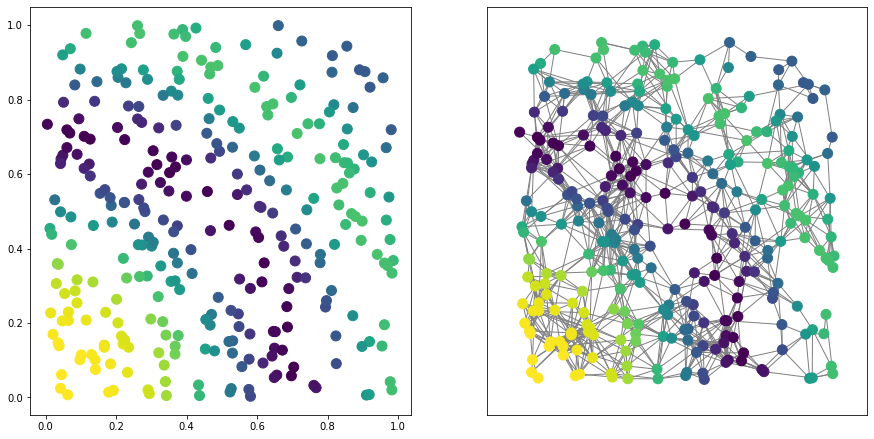
\includegraphics[width=0.8\textwidth]{lpm_image_correct.png}
    \caption{Left- latent positions, Right - Latent Position Random Graph}
    \label{fig:my_label}
    \end{figure}


\end{block}
\begin{block}{Main result: \myemphBLACK{A Sharp Variance Bound}}
LLN heuristics: by setting $b_n(f,x)=\dfrac{\int f(z)k_n(x,z)p(z)dz}{\int k_n(x,z)p(z)dz}$ we have 
\begin{equation*}
    \hat{f}_{GNW}(x)\sim b_n(f,x)
\end{equation*}
\vspace{10pt}
Suprisingly, we can compute
\begin{equation*}
    \mathbb{E}(\hat{f}_{GNW}(x))=b_n(f,x)(1-(1-\frac{d_n(x)}{n})^n)
\end{equation*}
We focus on bounding $\mathbb{E}(\hat{f}_{GNW}(x)-b_n(f,x))^2$ instead of $\mathbb{V}(\hat{f}_{GNW}(x))$
\vspace{10pt}
\mycolbackwhite{\textbf{Theorem}
    \vspace{10pt}
    \\
    If $f\colon\mathbb{R}^d\to\mathbb{R}$ is s.t. $||f||_{\infty}\leq B$ and $\mathbb{E}(\epsilon_1^2)=\sigma^2$. 
    Then
    \begin{equation*}
        \frac{\sigma^2(1-e^{-d_n(x)})}{d_n(x)}\leq \mathbb{E}(\hat{f}_{GNW}(x)-b_n(f,x))^2\leq \frac{C(B,\sigma^2)}{d_n(x)}
    \end{equation*}
    }
    \vspace{20pt}
    \begin{itemize}
        \item \textit{As soon as $d_n(x)\to\infty$, the \textit{variance term} tends to $0$} 
        \item \textit{Left to bound $|b_n(f,x)-f(x)|$ (the \textit{bias} term)} %\hspace*{\fill}{\textcolor{ForestGreen}{EASY}\qquad}
        \item  $d_n(x)\sim nh_n^dp(x)$ (\textit{Lebesgue Density theorem})
    \end{itemize}
    \begin{figure}
        \centering
        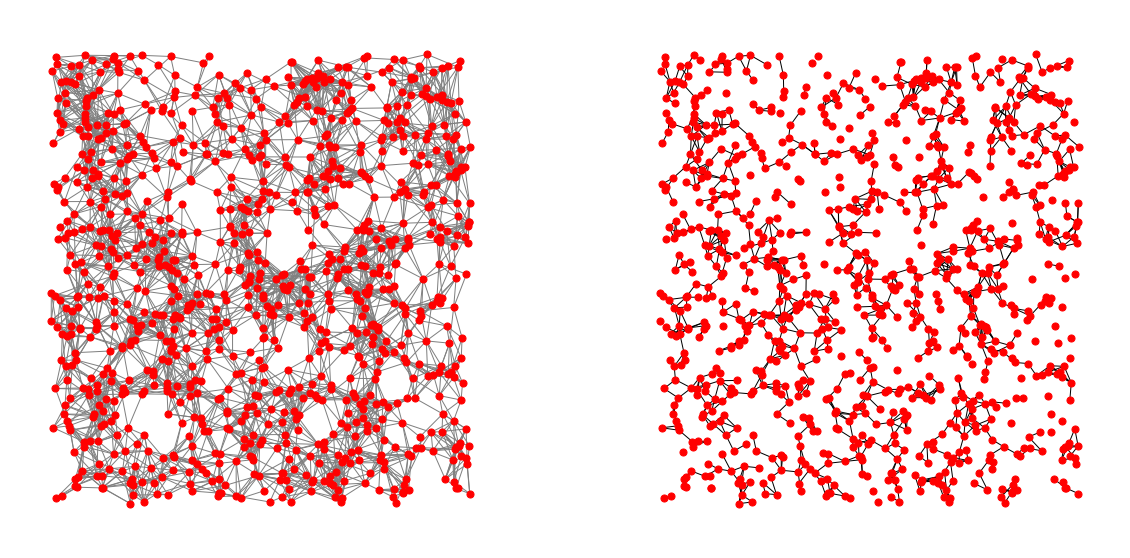
\includegraphics[width=0.8\textwidth]{fresh_for_marseille.png}
        \caption{Sparse random graphs. Left: $d_n(x)\sim\log(n)$, Right: $d_n(x)\sim\log(\log(n))$}
    \end{figure}
\end{block}

\begin{block}{\textit{Outlooks}}
    \begin{itemize}
        \item Signal estimation via \textbf{recovered} latent positions
        \item Guarantees for other \textbf{nonspectral} estimators
        \item Guarantees for \textbf{GNNs}
    \end{itemize}
\end{block}
\end{column}

%%%% Second Column

\begin{column}{0.49\textwidth}
\begin{block}{The \myemphr{NW} and \myemphh{GNW} estimators}
When the positions $X_1,....X_n$ are known, a popular approach is \myemphr{Nadaraya-Watson} Estimator
\begin{equation*}
    \hat{f}_{NW}(X)=\frac{\sum_{i=1}^n Y_iK(\frac{X-X_i}{h_n})}{\sum_{i=1}^n K(\frac{X-X_i}{h_n})}
    \end{equation*}
In the LPM setting, we consider 
\myemphh{Graphical Nadaraya-Watson} Estimator
    \begin{equation*}
        \hat{f}_{GNW}(X)=\frac{\sum_{i=1}^n Y_i a(X,X_i)}{\sum_{i=1}^n a(X,X_i)}
    \end{equation*}

The $L^2$ risk of the \myemphr{NW} estimator admits the bias-variance decomposition 
\vspace{10pt}
\begin{equation*}
    \mathbb{E}(\hat{f}_{NW}(x)-f(x))^2=\mathbb{V}(\hat{f}_{NW}(x))+(\mathbb{E}(\hat{f}_{NW}(x))-f(x))^2
\end{equation*}
\mycolbackgreenw{\textbf{Questions}
\vspace{10pt}
\begin{center}
    \begin{enumerate}
        \item How does the quality of $\hat{f}_{GNW}$ depend on the degree ?
        \vspace{10pt}
        \item How does the $L^2$ risk of $\hat{f}_{GNW}$ compare to that of $\hat{f}_{NW}$?
    \end{enumerate}
\end{center}
}
\end{block}
\begin{block}{Proof Sketch - the Decoupling trick}
   \small For $I\subseteq [n]$. Define\footnote{with the convention that $1/0=0$}  
    \small \begin{equation*}
        R_I(x)=
        \frac{1}{|I|+\sum_{j\notin I}a(x,X_i)}
    \end{equation*}
    \small For all pairs of \textbf{disjoint} subsets $I,J\subseteq$[n] we have
    \begin{equation*}
    R_J(x)\prod_{i\in I}a(x,X_i)=R_{I\cup J}(x)\prod_{i\in I}a(x,X_i)
    \end{equation*}
    \small and $R_{I\cup J}(x)$ is \textbf{\textit{independent}} from $\{a(x,X_i)|i\in I\}$.
    \vspace{20pt}
    \begin{itemize}
        \small \item "linearized" representation 
     $\hat{f}_{GNW}(x)=\sum_{i=1}^nY_ia(x,X_i)R_i(x)$ 
        \small \item concentration inequalities
    \end{itemize}
\end{block}
\begin{block}{MISE bound for convolutional kernels}
    Convolutional kernels $k_n(x,z)=K(\frac{x-z}{h_n})$ with $K\colon\mathbb{R}^d\to [0,1]$, $h_n>0$
    \mycolbackwhite{\textbf{Theorem}
    \vspace{10pt}
    \begin{itemize}
        \item $K$ compactly supported 
        \item $p(x)\geq p_0>0$ on $Q$ and $Q$ \textit{satisfies \myemph{interior cone condition}}
        \item f is \textit{$\alpha$ Hölder continnous on $\supp{p}$}
    \end{itemize}
    then for sufficiently small bandwiths $h_n$ we have
        \begin{equation*}
            \mathbb{E}(\hat{f}_{GNW}(X)-f(X))^2\leq C_1(\alpha)h_n^{\alpha}+\frac{C(B,\sigma)}{nh_n^d}
        \end{equation*}}
\end{block}


\begin{block}{Simulations}
    \begin{figure}
        \centering
        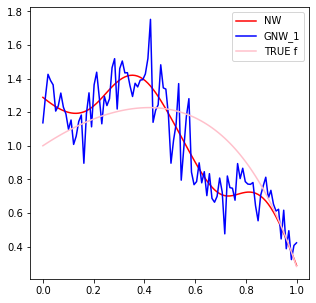
\includegraphics[width=0.3\textwidth]{trueSMALLsample.png}
        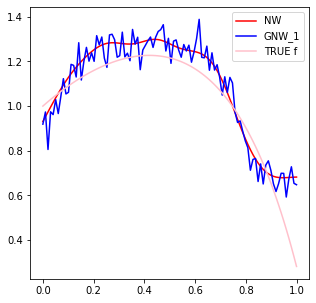
\includegraphics[width=0.3\textwidth]{trueMEDsample.png}
        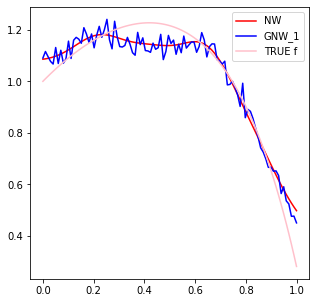
\includegraphics[width=0.3\textwidth]{trueLARGEsample.png}
        \caption{\myemphr{NW} vs \myemphh{GNW} estimators: Left- sample size n=100, center- sample size= 500mm right- sample size n=2000}
    \end{figure}
    
\end{block}



\begin{block}{References}
    {\footnotesize
    \begin{itemize}
    \item[{[1]}] B. Tsybakov. \textbf{Introduction to Nonparametric Estimation.} 1st.
    Springer Publishing Company
    \item[{[2]}] Vershynin. \textbf{High-Dimensional Probability: An Introduction with Applications in Data Science}. Cambridge University Press, 2018
    \item[{[3]}] [HRH02] Peter D Hoff, Adrian E Raftery, and Mark S Handcock. \textbf{Latent Space Ap-
    proaches to Social Network Analysis}. Journal of the American Statistical
    Association 97.460 (2002)
    \end{itemize}
    }
\end{block}
\end{column}
\end{columns}
\end{frame}
\end{document}